
As previously mentioned, curated data undergoes a distinct processing pipeline. This is due to the assumption that curated datasets generally maintain a higher level of quality, thereby requiring less intensive filtering and deduplication compared to web data. A comprehensive list of the curated datasets used in our study is provided in Table \ref{tab:curated_data_list}, which details 75 datasets, including information on language, format, license, domain, and the number of documents/words, along with the filtering percentage. In the subsequent sections, we will conduct a detailed analysis of the most significant columns.



\begin{figure}
    \centering
    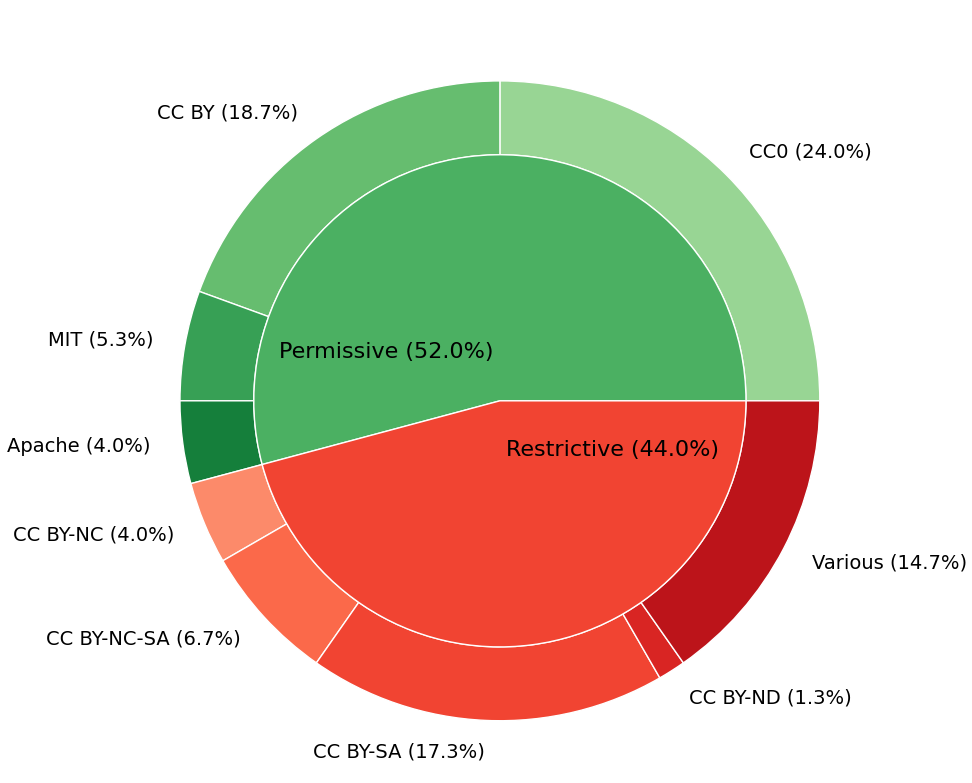
\includegraphics[width=0.6\linewidth]{images/Analysis/licenses.png}
    \caption{\label{fig:licenses}%
    Distribution of curated dataset licenses. Most datasets have permissive licenses (CC0, CC BY, MIT, Apache), 
    while restrictive licenses are primarily represented by datasets sourced from multiple origins (\textit{Various}). }
    
\end{figure}
\subsubsection{Licenses} 
As outlined in the data selection process (see Section \ref{sec:datasets.selection.curated}), selecting datasets according to legal and licensing constraints is a crucial first step. Figure \ref{fig:licenses} illustrates the distribution of licenses across the curated
%%comment: happened as an afterthought, not first step
datasets used in this project. The majority (52\%) of the selected datasets' licenses are permissive and not restricted for commercial use, featuring licenses like CC0 (24\%), CC BY (18.7\%), MIT (5.3\%), and Apache (4\%)\footnote{To simplify aggregation, the license versions are omitted here and in Figure \ref{fig:licenses}. However, in Table \ref{tab:curated_data_list}, the specific version numbers for all the datasets are clearly indicated.}. These licenses enable broad usage of the data, including for commercial purposes, and promote ease of dissemination and integration in various projects.

Conversely, 44\% of the datasets are categorized under restrictive licenses, which limit their use, especially for commercial applications. These include licenses such as CC BY-NC-SA (6.7\%), CC BY-NC (4\%), and the ``Various'' category (14.7\%), which represents datasets compiled from multiple sources and classified under the most restrictive license to mitigate legal risks. 


An important observation is that many datasets did not explicitly mention a license on their official website. For these datasets, we conducted further investigation into the sources, often uncovering related licensing information. However, for some datasets (marked with a dagger in Table \ref{tab:curated_data_list}), we were unable to directly determine the correct licenses despite extensive efforts. 
%In such cases, we made conservative assumptions, classifying them under the license most likely to be applicable based on related materials such as associated code or website. \todo{lennard: Just to be sure, we mean that default copy right laws apply, dont we? Because saying that we assumed the licence could be misleading}


\subsubsection{Languages}
\begin{figure}
\centering
\begin{subfigure}{.5\textwidth}
  \centering
  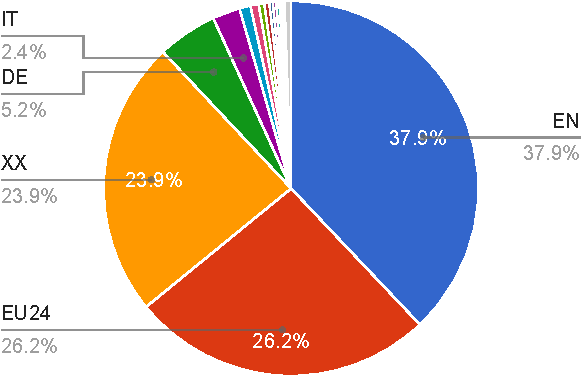
\includegraphics[width=0.95\linewidth]{images/Analysis/curated_lang_words_main.pdf}
  \caption{Complete word distribution} 
  \label{fig:curated_lang_word_a}
\end{subfigure}%
\begin{subfigure}{.5\textwidth}
  \centering
  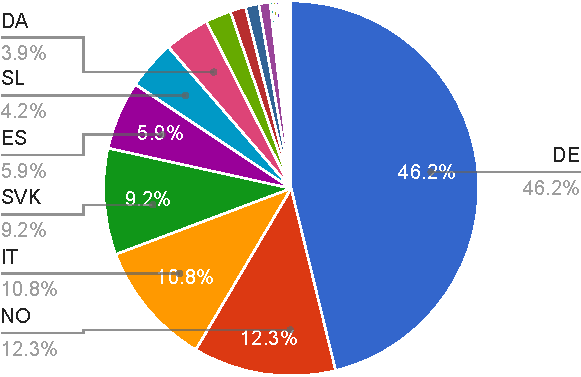
\includegraphics[width=0.95\linewidth]{images/Analysis/curated_lang_words_sub.pdf}
\caption{Word distribution excluding EN, EU24, and XX.}
\label{fig:curated_lang_word_b}
\end{subfigure}
 \caption{Word distribution across different languages in the curated datasets.}
\label{fig:curated_lang_word}
\end{figure}


Our curated dataset encompasses 24 unique languages. For clarity, datasets that include a substantial portion of the official 24 EU languages are grouped under the category “EU24”. Additionally, the analysis also features statistics for other European languages, such as Norwegian (NO). The label “XX” is used to indicate datasets focused on source code.

As shown in Figure \ref{fig:curated_lang_word_a}, English (EN) accounts for 37.9\% of the total word count, followed by the EU24 languages at 26.2\%, and source code (XX) at 23.9\%. Together, these three categories make up 88\% of the curated data. The inclusion of source code is particularly important in this context, as it provides curated, high-quality examples for training models on coding tasks.

Since many datasets feature multiple languages, specific per-language statistics are not always provided, but rather an overall distribution is emphasized.  On average, multilingual datasets contain significantly fewer words (712.8 million) compared to monolingual (4.38 billion) ones. Indeed,  while contributing to language diversity, they often lack the volume of content found in larger monolingual datasets.

After removing the dominant categories (EN, EU24, and XX), Figure \ref{fig:curated_lang_word_b} reveals that German (DE) constitutes 46.2\% of the remaining data. This significant proportion reflects the regional focus of the project, as it is based in Germany, and emphasizes the role of localized datasets in shaping the overall corpus. Other notable languages include Norwegian, Italian, and Spanish, though their contributions remain relatively smaller compared to German.



% Graph values
% Words per language
%EN EU24 XX DE NO IT SK ES SL DA PL FR MA ET BG HR RO HU SK GA EL LT BS MK SQ TR FI
%111512165187.44444 79951548548.0 73064206834.0 10956303105.666666 2920299614.0 2558626263.6666665 2174828161.0 1406434980.5 1007129655.7142857 922700245.0 525519997.71428573 317726618.3333333 276204170.0 227978247.0 61023899.82539683 61023899.82539683 61023899.82539683 53326169.71428572 53326169.71428572 44193174.0 36489045.11111111 23659959.5 7697730.111111111 7697730.111111111 7697730.111111111 7697730.111111111 3650602.0

\paragraph{Analysis of Word Distribution and Dataset Representation in Multilingual Corpora}
One would expect the word distribution to follow the number of datasets available; however, correlation analysis reveals this is only partially true. The Spearman correlation is moderate (0.562, p = 0.0028), while the Pearson correlation indicates a stronger linear relationship (0.855, $P < 0.001$). 
By using linear regression, we observe notable deviations in certain languages. For instance, German (DE) exhibits a significant negative residual, with the actual word count being 5.1 billion fewer than expected, despite having a high number of diverse datasets. This suggests that while German datasets are numerous, they tend to be smaller in size or less word-dense compared to other languages. On the other hand, English (EN) has a positive residual, showing 3.88 billion more words than predicted, which can be attributed to the oversampling of English datasets in the corpus. In contrast, French (FR) underperforms relative to its dataset count, with a negative residual of 1.54 billion, indicating that the French data is underrepresented in terms of word volume.

This analysis underscores the need for balanced sampling across languages. While oversampling English may provide more content for model training, undersampling key languages like French could result in biases that limit the multilingual capabilities of the models. Hence, we recommend strategic oversampling of underrepresented languages and careful moderation of overrepresented languages to ensure linguistic diversity and fairness in the curated dataset.


\subsubsection{Domains}

\begin{table}
\centering
\begin{tabular}{lrrrr}
\hline
Domain                 & \# Datasets & Avg. Words/DS [M] & Total Words [M] & Percentage [\%] \\ \hline
Source Code            & 1        & 73.064                & 73.064      & 40.46           \\
Law and Administration & 22       & 1.674                 & 36.839      & 20.40           \\
Web                    & 6        & 4.120                 & 24.721      & 13.69           \\
Medical                & 5        & 3.229                 & 16.147      & 8.94            \\
Math                   & 6        & 2.684                 & 16.105      & 8.92            \\
Forum                  & 2        & 3.655                 & 7.311       & 4.05            \\
Books                  & 5        & 752                   & 3.763       & 2.08            \\
News                   & 4        & 473                   & 1.893       & 1.05            \\
Knowledge Base         & 4        & 105                   & 423         & 0.23            \\
Culture                & 3        & 48                    & 146         & 0.08            \\
Recreation             & 2        & 73                    & 146         & 0.08            \\ \hline
\end{tabular}
\caption{Total words, average words per dataset (Avg Words/DS), and documents for each domain, sorted by total words. }
\label{tab:word_distribution_per_domain}
\end{table}

The curated dataset spans multiple domains, each contributing a different share to the total word count. Table \ref{tab:word_distribution_per_domain} provides a breakdown of the number of datasets, the average word count per dataset, total word count, and the percentage contribution of each domain.

Source code emerges as the largest domain by word count, accounting for 40.46\% of the total curated data, with over 73 billion words. This is followed by law and administration, which contributes 20.40\%, and the web domain at 13.69\%. Collectively, these three domains represent 74.55\% of the total word count. This strong presence of technical, legal, and digital content suggests that the curated dataset is well-suited for training models focused on tasks related to programming, legal reasoning, and web-based applications.

On the other hand, smaller domains such as culture (0.08\%), recreation (0.08\%), and knowledge base (0.23\%) contribute much less to the overall dataset. These domains are likely underrepresented either due to the limited availability of datasets or their inherently smaller size. 


\subsubsection{Sizes}

The distribution of word counts within the curated dataset is highly skewed, with a few large datasets contributing the majority of the total word volume as shown in Figure \ref{fig:curated_size}. Initially, the largest contributors were \textit{StarCoder}, \textit{EurLex}, and \textit{MaCoCu}, together accounting for 50\% of the total word count. However, since \textit{StarCoder} focuses on source code rather than natural language, it was excluded from further analysis, and the word count distribution was recalculated.

In the revised analysis, four datasets (\textit{peS2o}, \textit{MaCoCu}, \textit{Legal MC4}, and \textit{EurLex}) now make up 50\% of the total word count. Expanding this to 70\%, the dataset contributions broaden to include three additional Pile subsets (\textit{PMC extracts}, \textit{Openwebtext2}, and \textit{Free Law Opinions V2}), as well as \textit{Wikimedia Wikipedia}. Notably, 17 datasets account for 90\% of the total word count, underscoring the significant concentration of data within a limited number of large datasets.

\begin{figure}
    \centering
    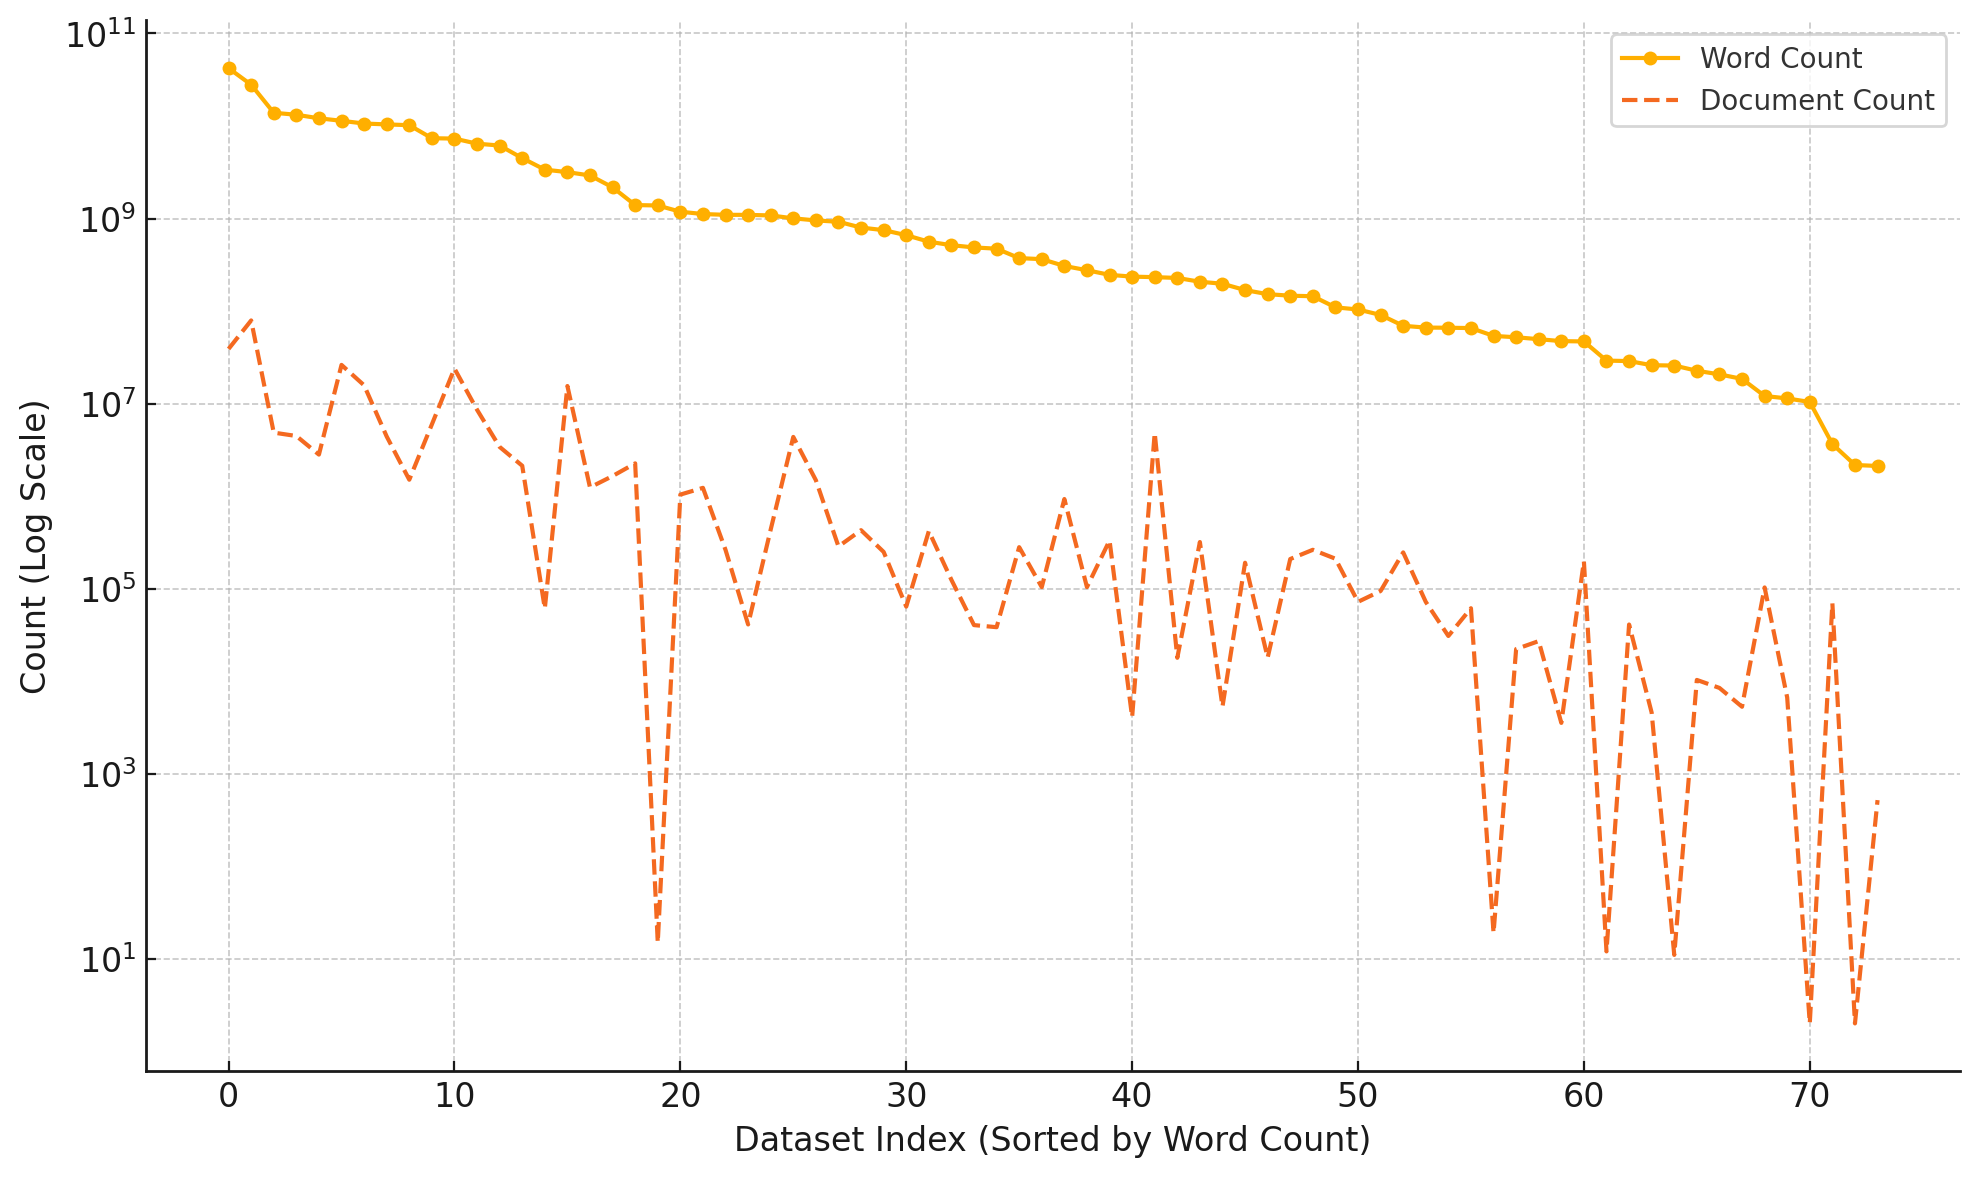
\includegraphics[width=0.7\linewidth]{images/Analysis/curated_size_log.png}
 \caption{Log-scaled comparison of word counts and document counts across datasets, sorted by word size. Some datasets exhibit a notably high word count despite having relatively few documents, indicating longer average document sizes.}    \label{fig:curated_size}
\end{figure}

Additionally, certain datasets display an unusually high word count relative to their document counts. A regression analysis was performed to better understand these discrepancies, calculating residuals to detect significant deviations from the expected document-to-word ratio. This analysis revealed the following outliers:

\begin{itemize} 
\item \textit{Spanish legal corpora (ES)}: This legal corpus consists of only 15 documents but contains over 1.38 billion words. The residual analysis (5.4) shows that the word count is approximately 221 times higher than expected based on the number of documents. This suggests that individual documents within this corpus are unusually large.

\item \textit{Projekt Gutenberg (EU24)}: A well-known collection of books, \textit{Projekt Gutenberg} contributes over 3.37 billion words with only 60,912 documents. This results in a positive residual of 1.8, indicating that the dataset's word count per document is significantly higher than the regression model predicted. This observation aligns with expectations for book collections, as books typically contain more words per document compared to other formats such as articles or reports.

\item \textit{Pile: PMC extracts (EN)}: A medical dataset with 2.8 million documents and over 12.1 billion words, \textit{PMC extracts} exhibits a positive residual of 1.07. This indicates that the word count is significantly higher than predicted by the model. This is expected, as the dataset primarily contains full-length medical research articles, which are generally more detailed and content-rich compared to other document types.

\end{itemize}


\subsubsection{Filtering}

Across the curated datasets, the average filtering percentage is 5.33\% ($\pm 5.98\%$). Based on these values, filtering can be  split in three categories:

\begin{itemize}
    \item Low Filtering ($<1\%$): Datasets that underwent minimal filtering, typically because they contained well-structured, clean data to begin with. 
    
    \item  Medium Filtering (1\% to 11.31\%): The majority of datasets fall into this category, with moderate filtering applied to remove noise or short documents without heavily impacting the total word count. 
    
    \item  High Filtering (>11.31\%): Datasets with a high filtering percentage, indicating substantial noise or irrelevant content. 
\end{itemize}

In reviewing the impact of filtering, we found that documents with low language scores typically fall into one of four categories: i) mixed-language documents, ii) documents with conversion errors containing numerous special characters, iii) documents involving closely related languages (e.g., Croatian and Serbo-Croatian), and iv) documents in low-resourced languages where the content was misidentified as a different language. 

To further understand the impact of filtering across datasets, we explored potential correlations between the percentage of filtered data and several key dataset characteristics: the number of words, number of documents, format, language, and domain. Our analysis showed only modest correlations in most cases, indicating that filtering tends to act somewhat independently of these factors (refer to Appendix \ref{sec:appendix.curated.filtering} for a more detailed analysis).


\subsubsection{Summary}
The curated dataset presents a comprehensive and diverse collection of 75 datasets spanning 25 languages, various domains, and multiple formats, offering a robust foundation for a wide range of research tasks. Despite some imbalances in distribution, particularly with large datasets dominating the total word count, the variety within the dataset makes it a valuable asset for training LLMs. The high presence of technical and legal data, alongside source code, reflects the strengths of this dataset in supporting tasks in these fields.

While filtering in general is necessary to ensure data quality, its impact on the curated datasets is relatively moderate, with only a few datasets requiring significant cleaning. The weak correlations found between filtering percentages and dataset characteristics suggest that filtering is driven more by the specificities of the dataset than by its size, format, or domain. 
In preparing data for training LLMs, we found that a strategic approach to selecting subsets is key. Leveraging the wide domain and language diversity can help ensure more balanced outcomes. 